\chapter{Methodology}

This chapter describes the architecture and methods that were needed in order to investigate the research questions presented in Section \ref{goals_and_research_questions}. An overview of the physical testbed will first be given, followed by the general setup for each machine and how the \gls{tcp} experimentation have been conducted using \gls{teacup}. \todo{expand}



\section{System Overview}

The objective of the system is to perform automated \gls{tcp} experiments. \todo{more...}




\subsection{The Raspberry Pi 3 Cluster}

The Raspberry Pi machine is a series of small single-board computers developed in the United Kingdom by the Raspberry Pi Foundation to promote teaching of basic computer science in schools and in developing countries. The Raspberry Pi 3 Model B+ was released in 2018, and is the model used in this cluster.

\begin{table}[H]
    \centering
    \begin{tabular}{ |p{4cm}|p{2cm}|p{4cm}|p{2cm}|p{2cm}|  }
        \hline
        \multicolumn{5}{|c|}{\textbf{Raspberry Pi 3 Model B+ Specifications}} \\
        \hline
        \textbf{CPU} & \textbf{RAM} & \textbf{NICs} & \textbf{Storage} & \textbf{USB}\\
        \hline
        Broadcom BCM2837B0 \newline Cortex-A53 (ARMv8) 64-bit SoC \newline 1.4GHz, Quad-core &
        1GB LPDDR2 SDRAM &
        Gigabit Ethernet over USB 2.0 \newline Dual IEEE 802.11ac WiFi, Bluetooth 4.2 &
        32GB Micro-SD &
        4 USB 2.0 ports\\
        \hline
    \end{tabular}
    \caption{The hardware specifications of Raspberry Pi 3 Model B+.}
\end{table}

The cluster consists of eight Raspberry Pi 3 Model B+ machines, all hooked up to a Zyxel switch. The switch provides interconnectivity, but also powers the machines through \gls{poe}.

\begin{figure}[H]
    \centering
    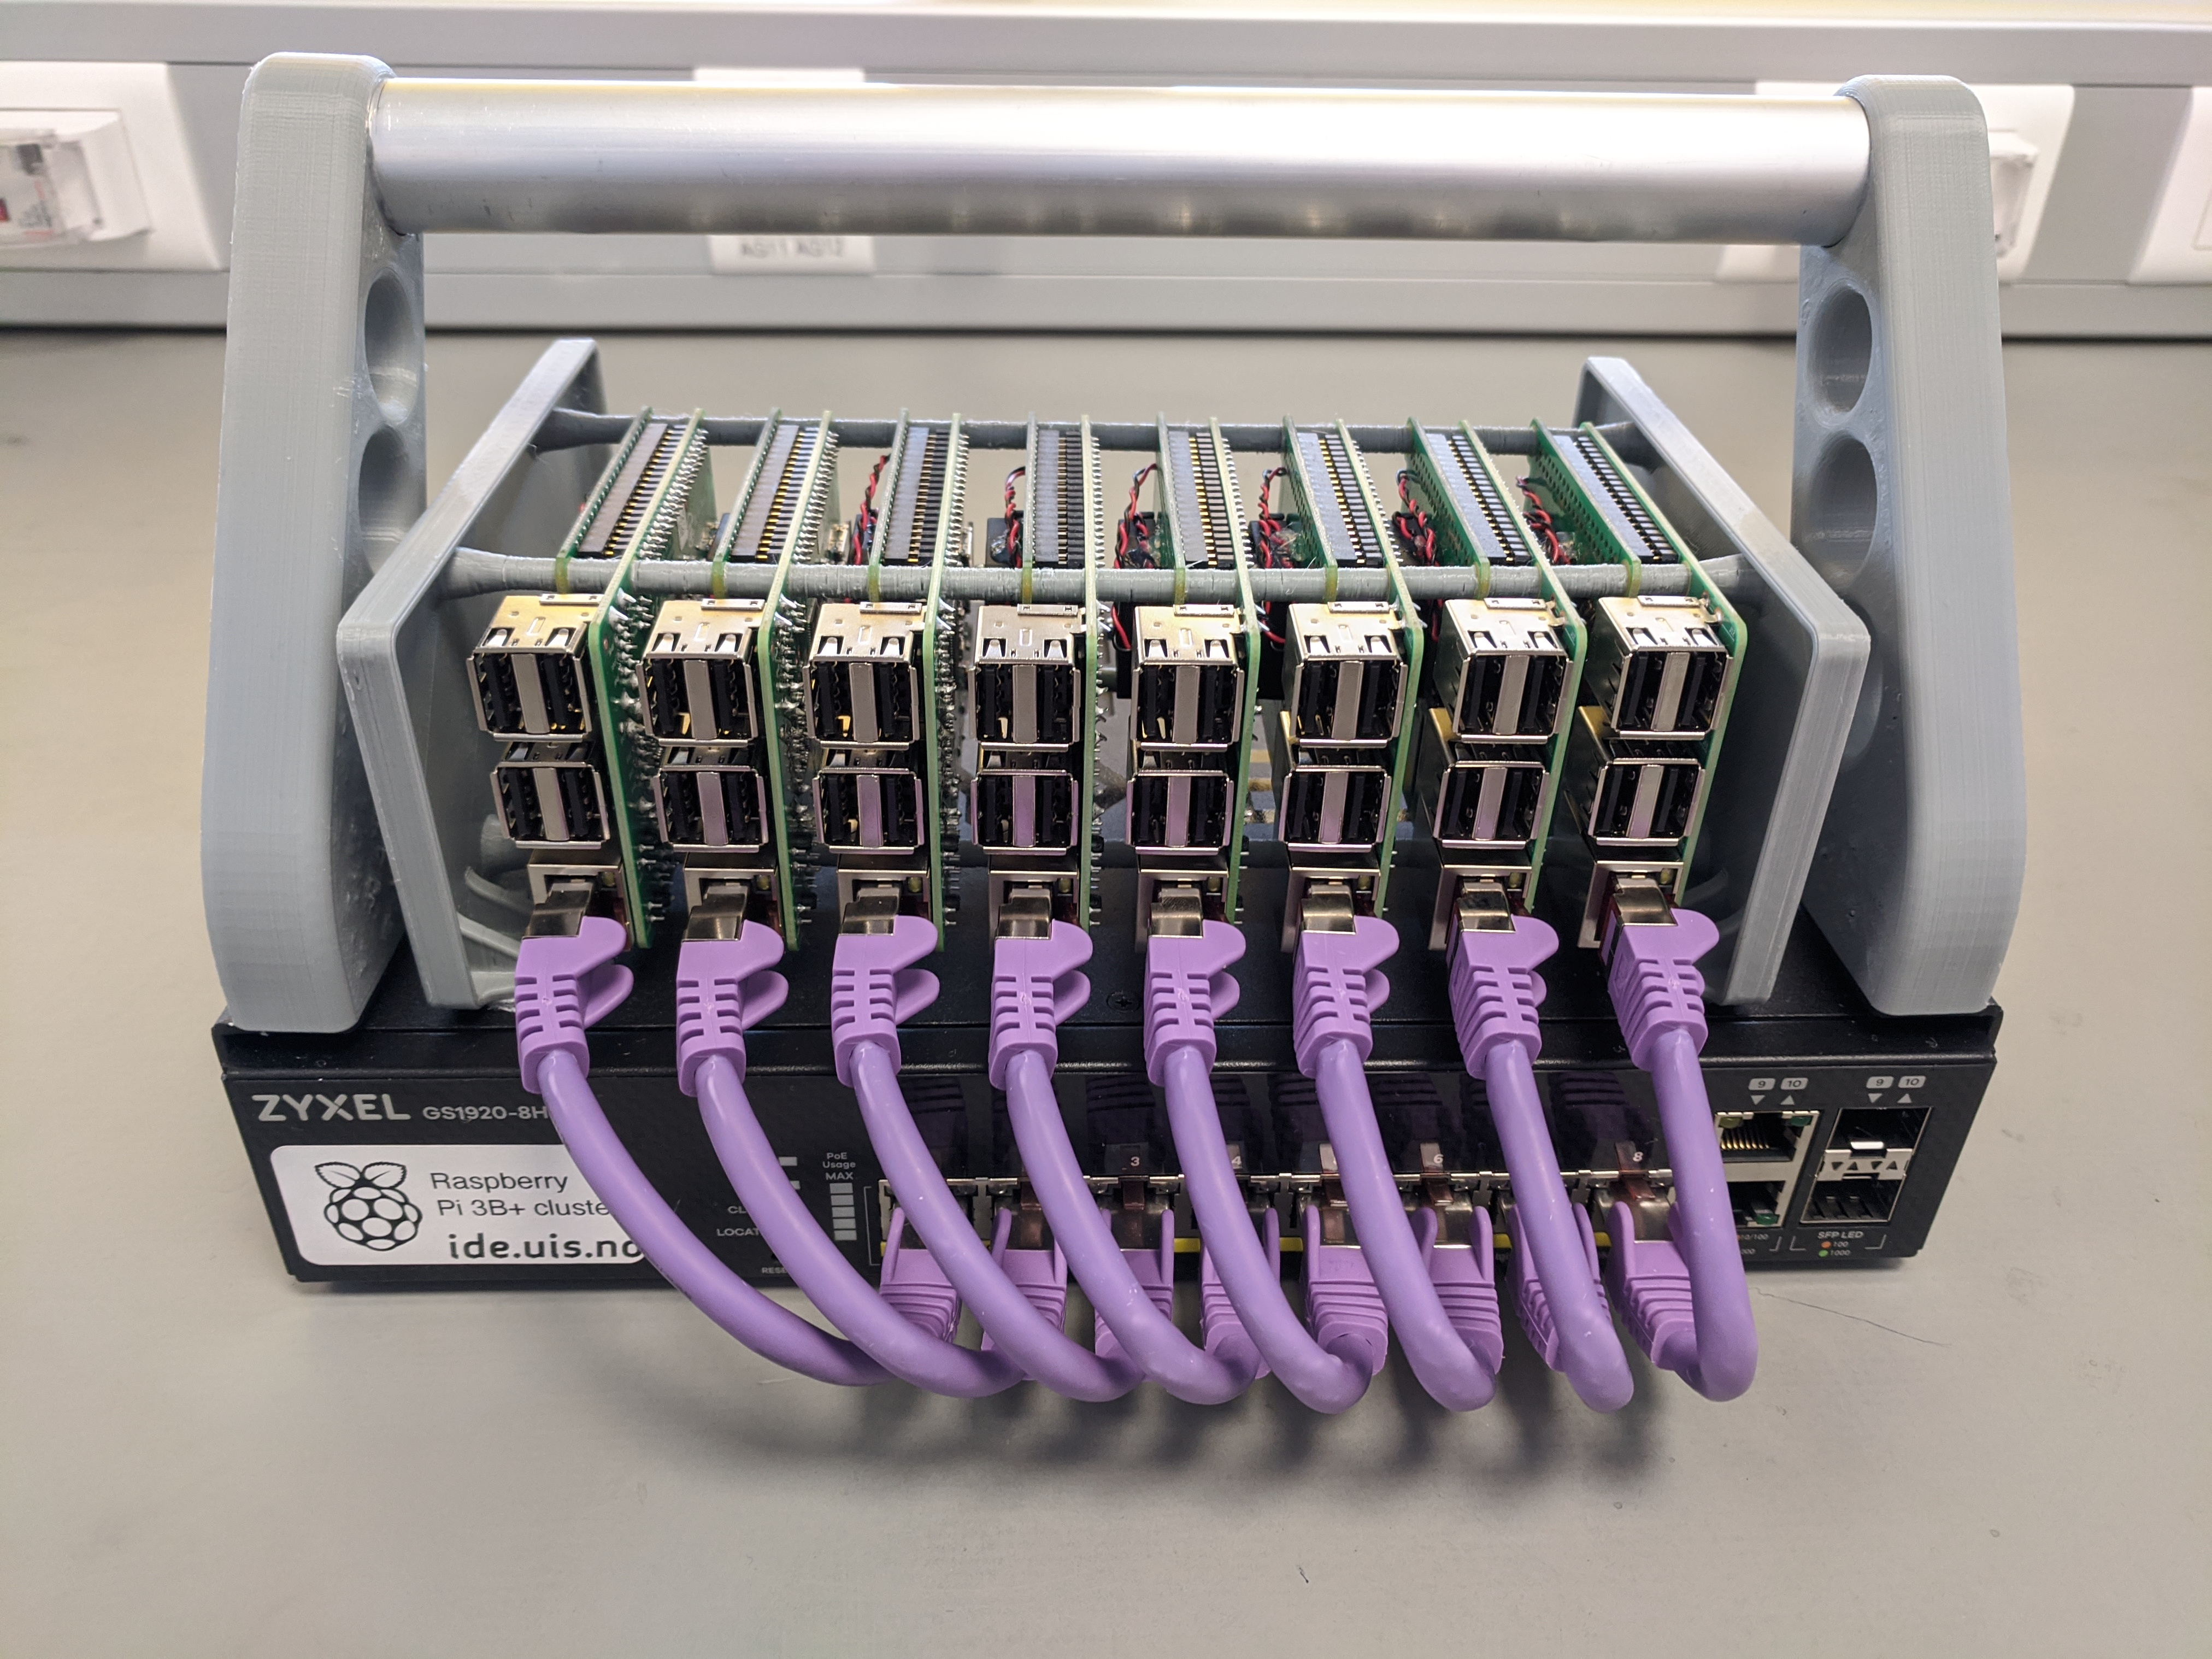
\includegraphics[width=0.6\linewidth]{pi3cluster}
    \captionsetup{width=0.6\linewidth}
    \caption{The Raspberry Pi 3B+ cluster all hooked to a Zyxel switch.}
    \label{fig:pi3cluster}
\end{figure}




\subsection{Network Topology} \label{network_topology}

The testbed consists of two networks; the \textit{controller} network in which all machines are connected directly, and the \textit{experimental} network separated by two subnets with a router in-between.

\begin{figure}[H]
    \centering
    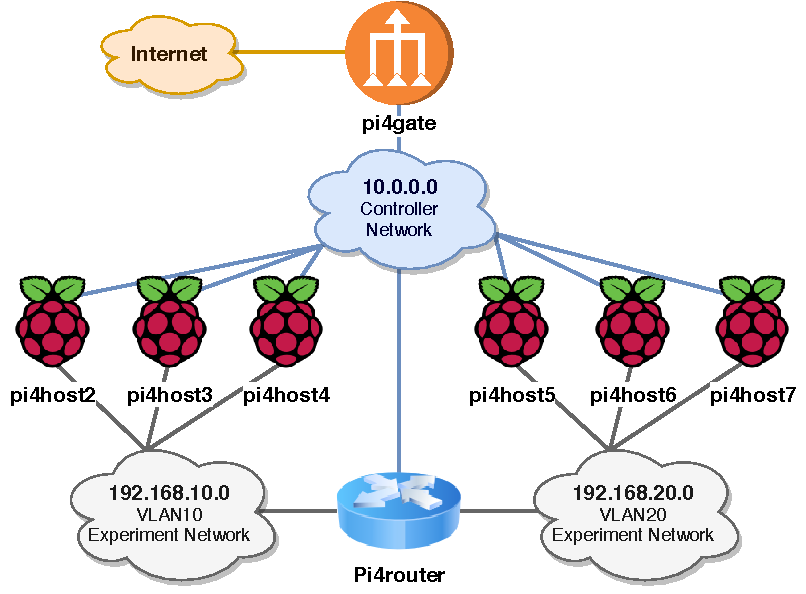
\includegraphics[width=0.8\linewidth]{network_topology}
    \captionsetup{width=0.8\linewidth}
    \caption{The logical network topology for the Raspberry Pi 3B+ cluster testbed.}
    \label{fig:network_topology}
\end{figure}

Since the entire testbed is connected to a single switch only, both \gls{vlan} and virtual interfaces have been used to achieve the desired network topology. In addition, one USB-to-ethernet adapter was necessary on the router in order to conduct network experimentation with \gls{teacup}. The \gls{vlan} setup on the switch is explained in section \ref{zyxel} while the general network setup for every machine is explained in the remaining sections.

A summary table of the network setup for each machine follows.

\begin{table}[H]
    \centering
    \begin{tabular}{ |p{2cm}|p{6cm}|p{3cm}|  }
        \hline
        \multicolumn{3}{|c|}{\textbf{Summary Network Setup}} \\
        \hline
        \textbf{Hostname} & \textbf{IP address} & \textbf{OS}\\
        \hline
        pi3router & 10.0.1.1 --- eth0 \newline 172.16.10.1 --- eth0:10 (virtual) \newline 172.16.20.1 --- eth1 (USB-to-eth) & Raspbian Buster (Linux)\\
        \hline
        pi3host2 & 10.0.1.2 --- eth0 \newline 172.16.10.2 --- eth0:10 (virtual) & FreeBSD 12.1\\
        \hline
        pi3host3 & 10.0.1.3 --- eth0 \newline 172.16.10.3 --- eth0:10 (virtual) & FreeBSD 12.1\\
        \hline
        pi3host4 & 10.0.1.4 --- eth0 \newline 172.16.10.4 --- eth0:10 (virtual) & FreeBSD 12.1\\
        \hline
        pi3host5 & 10.0.1.5 --- eth0 \newline 172.16.20.5 --- eth0:20 (virtual) & FreeBSD 12.1\\
        \hline
        pi3host6 & 10.0.1.6 --- eth0 \newline 172.16.20.6 --- eth0:20 (virtual) & FreeBSD 12.1\\
        \hline
        pi3host7 & 10.0.1.7 --- eth0 \newline 172.16.20.7 --- eth0:20 (virtual) & FreeBSD 12.1\\
        \hline
        pi3gate & DHCP --- eth0 \newline 10.0.1.254 --- eth0:1 (virtual) & Raspbian Buster (Linux)\\
        \hline
    \end{tabular}
    \caption{The hostnames, IP addresses and OS for each Raspberry Pi 3B+ machine in the cluster.}
\end{table}

The table above lists the configured Raspberry Pi 3B+ machines in left to right order as seen from \ref{fig:pi3cluster}. That is, the left most machine is set up as the router, and the right most machine is set up as the gateway.




\subsection{Zyxel GS1920-8HP} \label{zyxel}

The Zyxel GS1920-8HP model is a managed switch with 10 available ports for interconnectivity. The Zyxel switch is what powers every Raspberry Pi 3B+ machine using \gls{poe}, with port 9 providing Internet access.

\begin{figure}[H]
    \centering
    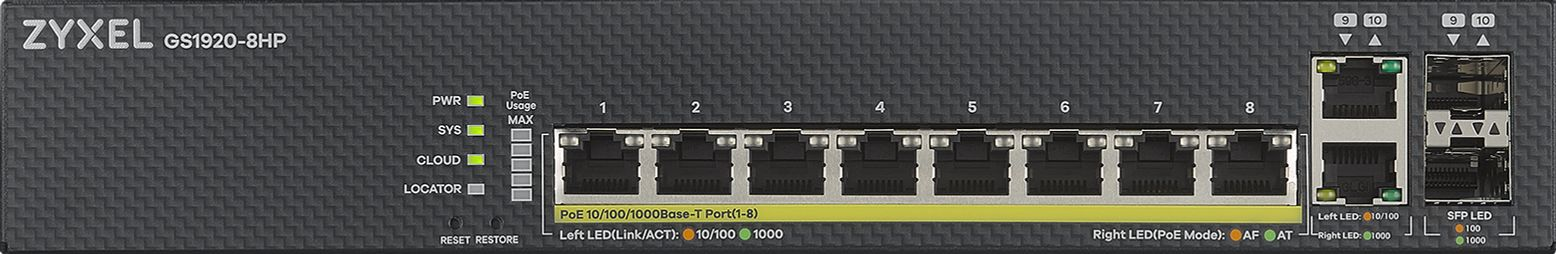
\includegraphics[width=1.0\linewidth]{zyxel}
    \captionsetup{width=1.0\linewidth}
    \caption{The front of the Zyxel GS1920-8HP managed switch.}
    \label{fig:zyxel}
\end{figure}

In order to logically separate two subnets on a single switch, as illustrated in \ref{fig:network_topology}, two \gls{vlan}s must be set up. This can easily be done through the switch's graphical user interface that can be accessed in several ways as shown in the official \href{https://www.zyxel.com/support/download_landing/product/gs1920_series_18.shtml?c=gb&l=en&pid=20130521174252&tab=Quick_Start_Guide&pname=GS1920%20Series}{quick start guide.}. In short, connect a computer to the Zyxel switch with an Ethernet cable, set a static IP of 192.168.1.10, and access the graphical user interface in a web browser by visiting the address 192.168.1.1.

The default username and password for Zyxel GS1920-8HP is \lstinline{admin} and \lstinline{1234}, respectively. Once logged in, go to \lstinline{Advanced Application -> VLAN -> VLAN Configuration -> Static VLAN Setup}.

\begin{figure}[H]
    \centering
    \begin{subfigure}{0.5\linewidth}
        \centering
        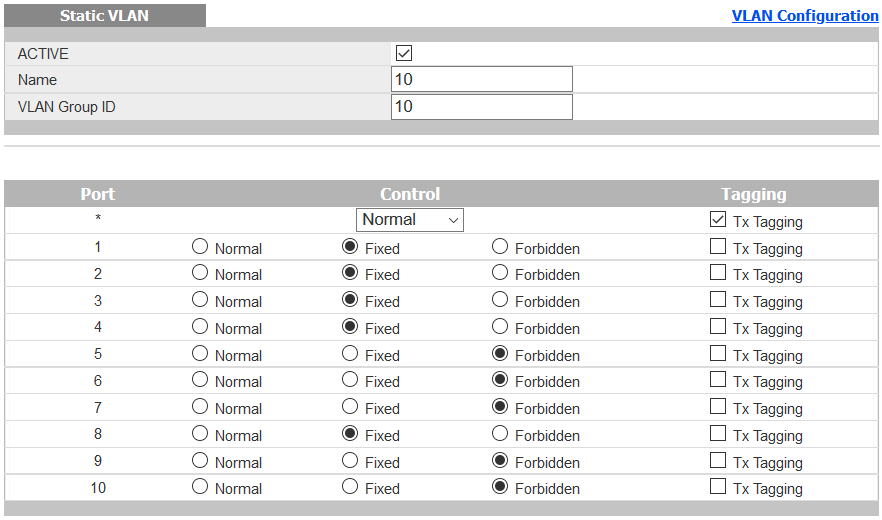
\includegraphics[width=1.0\linewidth]{vlan10}
        \caption{VLAN 10}
        \label{fig:vlan10}
    \end{subfigure}%
    \begin{subfigure}{0.5\linewidth}
        \centering
        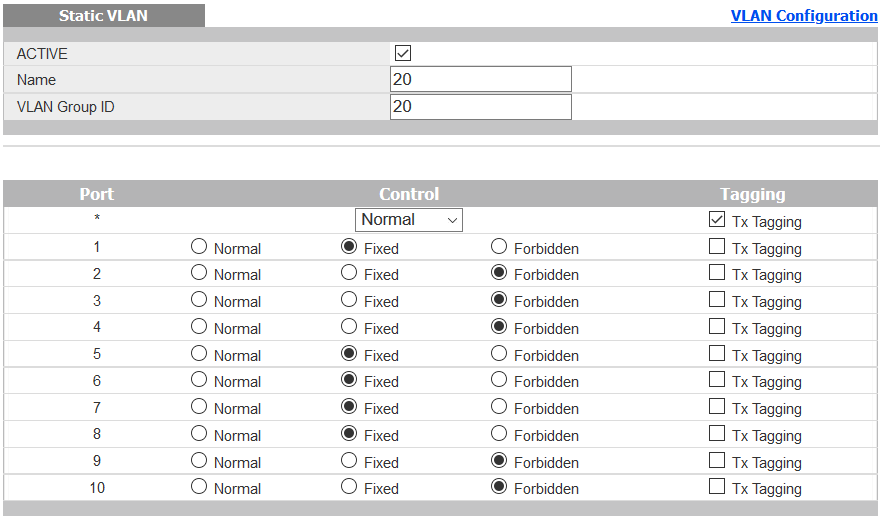
\includegraphics[width=1.0\linewidth]{vlan20}
        \caption{VLAN 20}
        \label{fig:vlan20}
    \end{subfigure}
    \caption{The configuration for the two \gls{vlan}s on Zyxel GS1920-8HP.}
    \label{fig:vlans}
\end{figure}

Create two \gls{vlan}s as shown above, confirming each creation with the \lstinline{Add} button. When done, persist the changes with the \lstinline{Save} button in the top right corner.




\section{General Setup}

This section serves as a guide for reproducing the general setup and configuration for the testbed. In the next sections, the following common tasks are assumed to have already been done on each Raspberry Pi 3B+ machine:

\begin{itemize}
    \item Installed an \gls{os} as specified in \ref{install_os}. Raspbian Buster is used on the gateway and router, and FreeBSD on the hosts.
    \item Changed the keyboard layout as specified in \ref{keyboard_layout}.
    \item Created a root user account as specified in \ref{root_account}.
    \item Updated the system as specified in \ref{update_system}.
    \item Enabled SSH as specified in \ref{enable_ssh}.
\end{itemize}

In addition, any given command is assumed to be run as \lstinline{root} user.

\subsection{Gateway}

This section describes how the machine with direct Internet access has been set up, known as the \textit{gateway}, and how it provides access and Internet for the other machines through \gls{nat}. The gateway is also known as the \textit{controller}, as this is where \gls{teacup} experiments are both configured and conducted from.


\subsubsection{Network}

The gateway is the only machine with direct Internet access through \gls{dhcp} on its main interface, with a virtual interface statically connected to the private controller network in order to communicate with the rest of the machines. To set up this, add the following to the \lstinline{/etc/network/interfaces} file:

\begin{minted}{bash}
# Main interface (Internet access)
auto eth0
iface eth0 inet dhcp

# Subinterface (controller-network)
auto eth0:1
iface eth0:1 inet static
address 10.0.1.254
netmask 255.255.255.0
\end{minted}

In order for the machines on the internal network to gain Internet access through the gateway, both \gls{ip} forwarding and \gls{nat} must be set up:

\begin{minted}{bash}
# Enable IP forwarding
echo 'net.ipv4.ip_forward=1' >> /etc/sysctl.conf

# NAT
update-alternatives --set iptables /usr/sbin/iptables-legacy
iptables -t nat -A POSTROUTING -o eth0 -j MASQUERADE
apt install iptables-persistent
\end{minted}

The hostname has also been changed to \lstinline{pi3gate} as specified in \ref{change_hostname}, followed by a reboot to apply all network changes.


\subsubsection{NTP Server}

\gls{teacup} requires that time is synchronized on all machines when running experiments. In order for the internal machines to synchronize their clock, an \gls{ntp} server must be set up. The gateway will provide this service, and is set up as specified in \ref{time_sync}.


\subsubsection{TEACUP} \label{teacup_gateway}

Every network experiment orchestrated by \gls{teacup} is initiated from the gateway, and so the majority of the tools for \gls{teacup} to work are installed on this machine. As described from the official \href{http://caia.swin.edu.au/tools/teacup/TEACUP-0.9_INSTALL.txt}{install} guide, with some slight adjustments, the following commands will install \gls{teacup} properly:

\begin{minted}{bash}
# R
apt install -y r-base

# PDFJAM
apt install -y texlive-extra-utils

# SPP
apt install -y mercurial libpcap-dev build-essential
hg clone https://bitbucket.org/caia-swin/spp
cd spp
make
mkdir /usr/local/man/man1
make install
cd ..

# Fabric
apt install -y fabric python-pip python-dev libffi-dev libssl-dev
pip install fabric3
pip install -Iv pexpect==3.2

# TEACUP
wget https://sourceforge.net/projects/teacup/files/teacup-1.1.tar.gz
tar -xf teacup-1.1.tar.gz
\end{minted}

To verify that \gls{teacup} has been properly installed, a simple check can be done as follows:

\begin{minted}{bash}
mkdir experiment
cp teacup-1.1/example_configs/config-scenario1.py experiment/config.py
cp teacup-1.1/run.sh experiment/
cp teacup-1.1/fabfile.py experiment/
\end{minted}

Go into the \lstinline{experiment} folder and prepare to edit the \lstinline{config.py} file. Find the line containing \lstinline{TPCONF_script_path = '/home/teacup/teacup-0.8'} and change the \lstinline{path} to where you extracted \lstinline{teacup-1.1}. Finally, verify \gls{teacup} installation with the command \lstinline{fab check_config}. If no errors appear, all is good.


\subsubsection{Modifications to TEACUP}

Due to the restricted physical set up as shown in \ref{fig:pi3cluster} and discussed in \ref{network_topology}, virtual interfaces have been used extensively, particularly on the router. This introduced a conflict to the \gls{teacup} codebase, as it assigns a name to each interface before performing network logging with \lstinline{tcpdump}. However, this name is not unique since both the controller and experiment network shares the same interface, resulting in a \lstinline{duplicate handle error} from \gls{teacup}. A slight adjustment to the codebase was therefore necessary.

Applying the following "band-aid" to the \lstinline{loggers.py} file in \gls{teacup} should fix the error:

\begin{minted}{bash}
--- teacup-1.1/loggers.py
+++ teacup-1.1-modified/loggers.py
@@ -41,6 +41,7 @@
    from getfile import getfile
    from runbg import runbg
    
+   import random
    
    ## Collect all the arguments (here basically a dummy method because we
    ## dont used the return value)
@@ -505,7 +506,7 @@
                    snap_len, interface, file_name, tcpdump_filter)
        pid = runbg(tcpdump_cmd)
    
-       name = 'tcpdump-' + interface
+       name = 'tcpdump-' + interface + str(random.randint(0, 50000))
        #bgproc.register_proc(env.host_string, name, '0', pid, file_name)
        bgproc.register_proc_later(
            env.host_string,
\end{minted}

In additon, a few changes to the \lstinline{hostsetup.py} file in \gls{teacup} must be done. \gls{teacup} checks if the \lstinline{sysctl} variable \lstinline{net.inet.tcp.reass.overflows} exists, which it does not for the FreeBSD version that we are using. The default sender and receiver buffer on FreeBSD hosts must also be set to a higher value, otherwise experiments would experience a capped \gls{cwnd} value. The changes are easily done as follows:

\begin{minted}{bash}
--- teacup-1.1/hostsetup.py
+++ teacup-1.1-modified/hostsetup.py
@@ -858,7 +858,7 @@
 
     if htype == 'FreeBSD':
         # record the number of reassembly queue overflows
-        run('sysctl net.inet.tcp.reass.overflows')
+        #run('sysctl net.inet.tcp.reass.overflows')
 
         # disable auto-tuning of receive buffer
         run('sysctl net.inet.tcp.recvbuf_auto=0')
@@ -869,6 +869,8 @@
         # send and receiver buffer max (2MB by default on FreeBSD 9.2 anyway)
         run('sysctl net.inet.tcp.sendbuf_max=2097152')
         run('sysctl net.inet.tcp.recvbuf_max=2097152')
+        run('sysctl net.inet.tcp.recvspace=655360')
+        run('sysctl net.inet.tcp.sendspace=327680')
 
         # clear host cache quickly, otherwise successive TCP connections will
         # start with ssthresh and cwnd from the end of most recent tcp
\end{minted}

Finally, the tool \lstinline{spp} does not run on the Raspberry Pi 3 or ARM architecture at all, only displaying the helpful message "\lstinline{aborting}" when running it. TEACUP uses this tool to calculate \gls{rtt}, and fortunately is only needed when analyzing the results. In other words, the experiment data can easily be copied over to an x86 machine where \lstinline{spp} works, and then be analyzed from there. That is, follow the install instructions above from \ref{teacup_gateway} again as normal, but on an x86 machine instead.






\subsection{Router}

This section describes how the router has been set up. \todo{maybe expand...}

\subsubsection{Network}

The router serves as the intermediate device for the hosts in order to conduct more realistic experiments. The main interface is statically connected to the controller network, with two additional interfaces (one virtual and one USB-to-eth) that function as the default gateway for the two separate subnets that the hosts reside in. To set the router up as such, add the following to the \lstinline{/etc/network/interfaces} file:

\begin{minted}{bash}
# Main interface (controller-network)
auto eth0
iface eth0 inet static
address 10.0.1.1
netmask 255.255.255.0
gateway 10.0.1.254

# Subinterface for VLAN 10 (experiment-network)
auto eth0:10
iface eth0:10 inet static
address 172.16.10.1
netmask 255.255.255.0
gateway 10.0.1.254

# USB-to-eth for VLAN 20 (experiment-network)
auto eth1
iface eth1 inet static
address 172.16.20.1
netmask 255.255.255.0
gateway 10.0.1.254
\end{minted}

In order for the hosts to communicate through the router, \gls{ip} forwarding must be enabled:

\begin{minted}{bash}
# Enable IP forwarding
echo 'net.ipv4.ip_forward=1' >> /etc/sysctl.conf
\end{minted}

The hostname has also been changed to \lstinline{pi3router} as specified in \ref{change_hostname}, followed by a reboot to apply all network changes.


\subsubsection{NTP Client}

To synchronize time for the router against the gateway, set the router up as an \gls{ntp} client as specified in \ref{time_sync}.


\subsubsection{TEACUP}

The router only needs two tools for \gls{teacup} to work properly when controlled from the gateway, and that is \lstinline{tcpdump} and \lstinline{ntp}:

\begin{minted}{bash}
# TEACUP tools on router
apt install -y tcpdump ntp
\end{minted}






\subsection{Hosts}

This section describes how each host has been set up. \todo{maybe expand...}


\subsubsection{Network}

The hosts are separated into two subnets. Hosts 2, 3 and 4 are on the network 172.16.10.0/24 (VLAN 10), while hosts 5, 6 and 7 are on 172.16.20.0/24 (VLAN 20). The main interface on each host is statically connected to the controller network, with an additional virtual interface (or \textit{alias} in FreeBSD) statically connected to the experimental network. To set up each host, run the following, but replace \lstinline{yy} with the appropriate \gls{vlan} and \lstinline{x} with the correct host number as illustrated in \ref{network_topology}:

\begin{minted}{bash}
# Main interface (controller-network)
echo 'ifconfig_ue0="inet 10.0.1.x netmask 255.255.255.0"' >> /etc/rc.conf
echo 'defaultrouter="10.0.1.254"' >> /etc/rc.conf

# Alias (experiment-network)
echo 'ifconfig_ue0_alias0="inet 172.16.yy.x netmask 255.255.255.0"' >> /etc/rc.conf
\end{minted}

In order for the hosts to communicate between each subnet, a static route must be added. Run the following to do so:

\begin{minted}{bash}
# Static route
echo 'static_routes="intnet"' >> /etc/rc.conf
echo 'route_intnet="-net 172.16.yy.0/24 172.16.xx.1"' >> /etc/rc.conf
\end{minted}

Replace \lstinline{yy} with the destination \gls{vlan} and \lstinline{xx} with the source \gls{vlan}.

The hostname has also been changed to \lstinline{pi3hostX} as specified in \ref{change_hostname}, where \lstinline{X} refers to the correct host number. A reboot will apply all network changes.


\subsubsection{NTP Client}

To synchronize time for each host against the gateway, set up each host as an \gls{ntp} client as specified in \ref{time_sync}.


\subsubsection{TEACUP}

\gls{teacup} requires four tools that must be installed on each host in order to run experiments, namely \lstinline{lighttpd},  \lstinline{iperf}, \lstinline{httperf} and \lstinline{nttcp}. The \lstinline{lighttpd} tool can be installed from the package repository with \lstinline{pkg install lighttpd}. A modified version of \lstinline{iperf} is used, and so must be installed from source as follows:

\begin{minted}{bash}
# Installing modified iperf on FreeBSD
wget https://sourceforge.net/projects/iperf2/files/iperf-2.0.9.tar.gz --no-check-certificate
tar -xf iperf-2.0.9.tar.gz
cd iperf-2.0.9
patch -p1 < iperf-2.0.9.patch
./configure
make
make install
\end{minted}

\todo{iperf-2.0.9.patch needs more explaining}

A modified version of \lstinline{httperf} is also used, but installing from source has proven unsuccessful. Thus, an unmodified version is therefore installed with \lstinline{pkg install httperf}. The last tool to install, \lstinline{nttcp}, is also modified, and so must be installed from source as follows:

\begin{minted}{bash}
# Installing modified nttcp on FreeBSD
wget http://caia.swin.edu.au/tools/teacup/downloads/nttcp-1.47-mod.tar.gz
tar -xf nttcp-1.47-mod.tar.gz
cd nttcp-1.47-mod
make
cp nttcp /bin/
\end{minted}


























\section{TCP Experimentation with TEACUP}




\section{Achieving Low Latency with ABE}



\section{Improving ABE}